\chapter{Higher (Second) Order Differential Equations \ode{}s}
Higher-order \ode{}s\index{\ode{}!higher order} often serve as models for mechanical and electrical systems, as 
relationships between position/velocity/acceleration and charge/current/voltage require multiple derivatives.

\section{Linear Equations}
A \textbf{linear differential equation of order $n$} is an equation of the form
\[
a_n(x) y^{(n)} + a_{n-1}(x) y^{(n-1)} + \cdots + a_1(x) y' + a_0(x) y = g(x),
\]
where the functions $a_0(x), a_1(x), \dots, a_n(x)$ and $g(x)$ are given, and $y$ is the unknown function.

If $g(x)=0$, the equation is called \textbf{homogeneous}. Otherwise, it is called \textbf{inhomogeneous}/\textbf{nonhomogeneous}.


\begin{definition}[Initial Value Problem]
  A \textbf{higher-order initial value problem (IVP)} specifies the values of the function and its derivatives at a single point.
  \begin{align*}
    \text{That is, } \quad & a_n(x) y^{(n)} + a_{n-1}(x) y^{(n-1)} + \cdots + a_1(x) y' + a_0(x) y = g(x),\\
    \text{Subject to} \quad & y(x_0) = y_0, \, y'(x_0) = y_1, \ldots, y^{(n-1)}(x_0)=y_{n-1}
  \end{align*}
\end{definition}


For a $2$nd-order equation, an IVP looks like
\[
y'' + p(x)y' + q(x)y = g(x), \quad y(x_0)=y_0, \; y'(x_0)=y_1.
\]

\begin{theorem}[Existence of a Solution]
  Let $a_0(x), a_1(x), \dots, a_n(x)$ and $g(x)$ be continuous on an interval \(I\), and let \(a_n(x)\neq 0\) for all \(x\in I\).
  If the initial condition \(x=x_0 \in I\), then a unique solution \(y(x)\) of the IVP exists.
\end{theorem}


\begin{definition}[Boundary Value Problems]
  A second-order \textbf{boundary value problem (BVP)} specifies the values of the function at two different points.
  \begin{align*}
    \text{That is,} \quad&  y'' + p(x)y' + q(x)y = g(x)\\
    \text{Subject to} \quad& y(a)=y_0, \; y(b)=y_1.
  \end{align*}
\end{definition}


\subsection{Homogeneous Equations}
  A linear homogeneous $n$-th order equation has the form
  \[
  a_n y^{(n)} + a_{n-1} y^{(n-1)} + \cdots + a_0 y = 0.
  \]


\begin{theorem}[Superposition Principle]
 Let \(y_1,y_2,\ldots,y_k\) be solutions of the \textcolor{cyan}{homogeneous} \(n\)th-order differential equation on an interval \(I\).
  Then the linear combination 
  \[
  y = c_1y_1(x) + c_2y_2(x) + \cdots + c_ky_k(x),
  \]
  where \(c_i\) are arbitrary constants, is also a solution on the \(I\).
\end{theorem}



\begin{example}
  Verify that the functions \(y_1 = x^2\) and \(y_2=x^2\ln\,x\) are both solutions of the homogeneous linear equation
  \(x^3y''' - 2xy' + 4y =0\) on the interval \((0, \infty)\).
  Show by the superposition principle that the linear combination is also a solution on the same interval
\end{example}



\begin{definition}[Linear Dependence/Independence]
  A set of functions \(\{f_1(x),f_2(x),\ldots,f_k(x)\}\) is said to be \textbf{linearly dependent} on an interval \(I\) if there exist constants
   \(c_1\neq c_2 \neq \ldots \neq c_k \neq 0\) such that
   \[
   c_1f_1(x) + c_2f_2(x) + \ldots + c_kf_k(x) = 0
   \]
   for every \(x\) in the interval.
   Otherwise, the set is \textbf{linearly independent}
\end{definition}

When finding solutions to linear differential equations, we are interested in linearly independent functions.
We can use a more "indirect" definition to check whether a set of functions is linearly independent.


\begin{definition}[Wronskian]
  Suppose that the set of functions \(\{f_1(x),f_2(x),\ldots,f_k(x)\}\) are \(k-1\) times differentiable.
  The determinant
  \[
    W(f_1, f_2, \dots, f_k)(x) =
    \begin{vmatrix}
    f_1(x) & f_2(x) & \cdots & f_k(x) \\
    f_1'(x) & f_2'(x) & \cdots & f_k'(x) \\
    \vdots & \vdots & \ddots & \vdots \\
    f_1^{(k-1)}(x) & f_2^{(k-1)}(x) & \cdots & f_k^{(k-1)}(x)
    \end{vmatrix}
  \]
  is called the \textbf{Wronskian} of the functions.
\end{definition}


\begin{theorem}[Criterion for Linearly Independent Solutions]
  Let \(y_1,y_2,\ldots,y_k\) be \(k\) solutions of the homogeneous linear \(n\)th-order differential equation
  \[
  a_n y^{(n)} + a_{n-1} y^{(n-1)} + \cdots + a_0 y = 0.
  \]
  on an interval \(I\).
  Then the set of solutions is linearly independent on \(I\) if \(W(y_1,y_2,\ldots,y_k)\neq 0\) for every \(x\) in the interval.
\end{theorem}


\begin{example}
  Verify that 
  \[
  y_1 = \frac{\cos{(2\ln\,x)}}{x^3} \quad \text{and} \quad y_2 = \frac{\sin{(2\ln\,x)}}{x^3}
  \]
  are linearly independent solutions of the differential equation \(x^2y'' + 7xy' + 13y = 0\) on the interval \(I = (0, \infty)\).
\end{example}


\begin{definition}[Fundamental Set of Solutions]
  A fundamental set of solutions of a homogeneous linear \(k\)th-order differential equation 
  \[
  a_k y^{(k)} + a_{k-1} y^{(k-1)} + \cdots + a_0 y = 0.
  \]
  on an interval \(I\) is any set of \(k\) linearly independent solutions \(\{y_1,y_2,\ldots,y_k\}\) on the interval \(I\).
\end{definition}


\begin{theorem}[General Solution of Homogeneous Equations]
   Let \(y_1,y_2,\ldots,y_k\) be a fundamental set of solutions of the homogeneous linear \(k\)th-order differential equation
   on the interval \(I\).
   Then the general solution of the equation on the interval is
   \[
   y = c_1y_1 + c_2y_2 + \cdots + c_ky_k,
   \]
   where \(c_i\) are arbitrary constants.
\end{theorem}




\subsection{Nonhomogeneous Equations}
A \textbf{nonhomogeneous linear equation} has the form
\[
a_n y^{(n)} + a_{n-1} y^{(n-1)} + \cdots + a_0 y = g(x).
\]

The general solution is
\[
y(x) = y_h(x) + y_p(x),
\]
where $y_h$ solves the homogeneous equation and $y_p$ is any \textbf{particular solution}.

Methods for finding $y_p$ include:
\begin{itemize}
    \item Method of undetermined coefficients (for exponential, polynomial, sine, cosine $g(x)$).
    \item Variation of parameters (general but more involved).
\end{itemize}


\begin{theorem}[General Solution of Nonhomogeneous Equations]
   Let \(y_p\) be any particular solution of the homogrneous linear \(k\)th-order differential equation on an interval \(I\), and
   let \(y_1,y_2,\ldots,y_k\) be a fundamental set of solutions of the associated homogeneous equation on the interval \(I\).
   Then the general solution of the equation on the interval is
   \[
   y = c_1y_1 + c_2y_2 + \cdots + c_ky_k + y_p,
   \]
   where \(c_i\) are arbitrary constants.
\end{theorem}

\newthought{Note:} there is an equivalent superposition principle for nonhomogeneous equations


\begin{example}
  Is \(y_p = -4x^2\) a particular solution of \(y'' - 3y' + 4y = -16x^2 + 24x - 8\)?
\end{example}


% ---

% \begin{question}
% Solve the following problems:
% \begin{enumerate}
%     \item Solve the IVP $y''+y=0, \; y(0)=0, \; y'(0)=1$.
%     \item Solve the homogeneous equation $y'''-3y''+3y'-y=0$.
%     \item Solve the nonhomogeneous equation $y''+y=\cos x$.
%     \item Formulate a boundary value problem for a beam deflection model involving $y''=f(x)$, and discuss the difference from an IVP.
% \end{enumerate}
% \end{question}



\section{Reduction of Order}
The \textbf{reduction of order} method is a technique used to find a 
second linearly independent solution to a second-order linear homogeneous ODE when one solution is already known.

Consider the equation
\[
y'' + p(x)y' + q(x)y = 0.
\]
Suppose $y_1(x)$ is a known solution. To find another solution, assume
\[
y_2(x) = v(x)y_1(x),
\]
where $v(x)$ is an unknown function. Substituting into the equation gives a first-order equation for $v'(x)$, which can then be solved.



\begin{example}
Solve
\[
y'' - y = 0,
\]
given that $y_1(x)=e^x$ is a solution.

\textbf{Solution.}  
Assume $y_2(x) = v(x)e^x$. Then
\[
y_2' = v'e^x + ve^x, \quad y_2''= v''e^x+2v'e^x+ve^x.
\]
Substitute into the ODE:
\[
(v''e^x+2v'e^x+ve^x) - (ve^x) = e^x(v''+2v')=0.
\]
So
\[
v''+2v'=0.
\]
Let $w=v'$, then $w'+2w=0$. Solution: $w=Ce^{-2x}$.  
Integrating:
\[
v=\int Ce^{-2x}\,dx = -\tfrac{C}{2}e^{-2x}+D.
\]
Thus
\[
y_2(x) = v(x)e^x = -\tfrac{C}{2}e^{-x}+De^x.
\]
A new independent solution is $y_2(x)=e^{-x}$.

So the general solution is
\[
y(x)=C_1 e^x + C_2 e^{-x}.
\]
\end{example}



\begin{question}
Given $y_1(x)=x$ is a solution of the ODE
\[
x^2y'' - 2xy' + 2y = 0,
\]
use reduction of order to find a second solution.
\end{question}




\section{Homogeneous Linear Equations with Constant Coefficients}
 
Characteristic\index{characteristic equation!higher order \ode{}s} equations\footnote{``Characteristic'' and ``auxiliary'' equations are used interchangeably here and in the textbook.
We will see that another characteristic equations will appear in matrix \ode{}s, and its roots are going to carry a similar interpretation.} 
help us solve higher-order linear \ode{}s whose parameters (coefficients) do not change. 
They convert a \ode{} into a polynomial equation, whose roots help us write down the solution.
As polynomials can have complex numbers as roots, we will have to learn basic complex number arithmetic.

\begin{highlight}
\subsection{Complex Numbers}
\textcolor{green!70}{Complex numbers}\index{complex numbers} \(z \in \mathbb{C}\) are specified using two (independent) real numbers (elements of \(\mathbb{R}\)).
There are two different representations of any complex number \(z\):

A complex number is of the form
\[
z = x + iy, \quad x,y \in \mathbb{R}, \; i^2=-1.
\]
\[
\Re(z)=x, \quad \Im(z)=y, \quad \mathbb{C} = \{x+iy: x,y\in \mathbb{R}\}.
\]

\section{Notations}
\begin{description}
    \item \textbf{Cartesian form:} $z = \Re z + i \Im z$. Components are called real and imaginary parts. \index{complex number!cartesian form}
    \item \textbf{Polar form:} $z = \abs{z} e^{i \arg(z)} = r(\cos\theta + i\sin\theta)$, with $r=|z|=\sqrt{x^2+y^2}$ and $\theta = \arg(z)$.
          Components are called magnitude (or modulus) and angle (or argument). \index{complex number!polar form}
    \item \textbf{Exponential form:} $z = re^{i\theta}$, using Euler’s formula $e^{i\theta}=\cos\theta+i\sin\theta$.
    \item \textbf{Trigonometric form:} $z = r(\cos\theta+i\sin\theta)$.
    \item \textbf{Matrix form:}
    \[
    z \equiv \begin{bmatrix} x & -y \\ y & x \end{bmatrix}.
    \]
    \item \textbf{Vector form:} $z = (x,y)$ in $\mathbb{R}^2$.
\end{description}

\textbf{Operations}

For $z_1=x_1+iy_1$, $z_2=x_2+iy_2$:
\[
z_1+z_2=(x_1+x_2)+i(y_1+y_2), \quad
z_1-z_2=(x_1-x_2)+i(y_1-y_2).
\]
\[
z_1z_2=r_1r_2e^{i(\theta_1+\theta_2)}, \quad
\frac{z_1}{z_2}=\frac{r_1}{r_2}e^{i(\theta_1-\theta_2)}.
\]
\[
\overline{z}=x-iy, \quad |z|=\sqrt{x^2+y^2}.
\]

\textbf{Exponential Function}:

The complex exponential function $e^z$ can be defined in several equivalent ways:

\textbf{1. Power Series Definition}
\[
e^z = \sum_{n=0}^\infty \frac{z^n}{n!}, \quad z\in\mathbb{C}.
\]

\textbf{2. Limit Definition}
\[
e^z = \lim_{n \to \infty} \left(1 + \frac{z}{n}\right)^n.
\]

\textbf{3. Differential Equation Definition}
$e^z$ is the unique function satisfying
\[
\frac{d}{dz} e^z = e^z, \quad e^0 = 1.
\]

\subsection*{4. Euler’s Formula (for purely imaginary arguments)}
\[
e^{i\theta} = \cos\theta + i\sin\theta, \quad \theta \in \mathbb{R}.
\]

These definitions are consistent and extend the exponential function naturally from $\mathbb{R}$ to $\mathbb{C}$.

\textbf{De Moivre's Theorem}
\[
\big(r(\cos\theta+i\sin\theta)\big)^n = r^n(\cos(n\theta)+i\sin(n\theta)), \quad n \in \mathbb{Z}.
\]

\textbf{Roots of Complex Numbers}
The $n$th roots of $z=re^{i\theta}$ are
\[
z_k = r^{1/n} e^{i\left(\frac{\theta+2k\pi}{n}\right)}, \quad k=0,1,\dots,n-1.
\]
\end{highlight}



A linear homogeneous differential equation with constant coefficients has the form
\[
a_n y^{(n)} + a_{n-1} y^{(n-1)} + \cdots + a_1 y' + a_0 y = 0,
\]
where $a_i$ are constants.

The method of solution:
\begin{enumerate}[\bfseries Step (1)]
    \item Form the \textbf{characteristic equation}:
    \[
      a_n r^n + a_{n-1} r^{n-1} + \cdots + a_0 = 0.
    \]
    \item Solve for the roots $r$.
    \item Build the general solution from the roots:
    \begin{itemize}
        \item Real distinct roots $r_1,\dots,r_n$:  
        $y(x) = C_1 e^{r_1 x} + \cdots + C_n e^{r_n x}$.
        \item Repeated root $r$ of multiplicity $m$:  
        $y(x) = (C_1 + C_2 x + \cdots + C_m x^{m-1}) e^{rx}$.
        \item Complex roots $r=\alpha \pm i\beta$:  
        $y(x) = e^{\alpha x}(C_1\cos \beta x + C_2\sin \beta x)$.
    \end{itemize}
\end{enumerate}



\begin{example}
Solve
\[
y'' + 4y' + 4y=0.
\]
\textbf{Solution.}  
Characteristic equation:
\[
r^2+4r+4=0 \quad \Rightarrow \quad (r+2)^2=0.
\]
Repeated root: $r=-2$ of multiplicity $2$.  
So the solution is
\[
y(x)=(C_1+C_2x)e^{-2x}.
\]
\end{example}



\begin{example}
Solve
\[
y''' - 3y'' + 3y' - y=0.
\]
\textbf{Solution.}  
Characteristic equation:
\[
r^3-3r^2+3r-1=0 \quad \Rightarrow \quad (r-1)^3=0.
\]
So root $r=1$ with multiplicity 3.  
General solution:
\[
y(x)=(C_1+C_2x+C_3x^2)e^x.
\]
\end{example}



\begin{question}
Solve the following equations:
\begin{enumerate}
    \item $y''-5y'+6y=0$
    \item $y''+9y=0$
    \item $y''' + y'' - y' - y = 0$
\end{enumerate}
\end{question}







\section{Method of Undetermined Coefficients: Superposition Approach}

Consider a linear nonhomogeneous differential equation with constant coefficients:
\[
L[y] = y^{(n)} + a_{n-1} y^{(n-1)} + \cdots + a_1 y' + a_0 y = g(x),
\]
where $L$ is a linear differential operator with constant coefficients.

\subsection*{Idea}
\begin{itemize}
    \item Solve the \textbf{homogeneous equation} $L[y]=0$ to get the complementary solution $y_c$.
    \item Find a \textbf{particular solution} $y_p$ by guessing a form similar to $g(x)$ (with undetermined coefficients).
    \item The general solution is $y(x)=y_c+y_p$.
\end{itemize}

\subsection*{Superposition Principle}
If
\[
L[y]=g_1(x)+g_2(x)+\cdots+g_k(x),
\]
then
\[
y_p = y_{p1}+y_{p2}+\cdots+y_{pk},
\]
where each $y_{pi}$ corresponds to a particular solution of $L[y]=g_i(x)$.

---

\begin{example}
Solve
\[
y'' - 3y' + 2y = e^x + \sin x.
\]

\textbf{Solution.}  
Homogeneous part:
\[
r^2-3r+2=0 \quad \Rightarrow \quad (r-1)(r-2)=0.
\]
So $y_c=C_1e^x+C_2e^{2x}$.

For $g(x)=e^x$: since $e^x$ already appears in $y_c$, guess
\[
y_{p1}=Ax e^x.
\]
Substitute:
\[
y_{p1}'=Ae^x+Ax e^x, \quad y_{p1}''=2Ae^x+Ax e^x.
\]
So
\[
y_{p1}'' - 3y_{p1}' + 2y_{p1} = (2Ae^x+Ax e^x) -3(Ae^x+Ax e^x)+2(Ax e^x).
\]
Simplify:
\[
= (2A-3A)e^x + (A-3A+2A)x e^x = -Ae^x.
\]
Set equal to $e^x$: $-A=1 \Rightarrow A=-1$.  
So $y_{p1}=-xe^x$.

For $g(x)=\sin x$: guess
\[
y_{p2}=A\cos x + B\sin x.
\]
Substitute:
\[
y_{p2}'=-A\sin x + B\cos x, \quad y_{p2}''=-A\cos x -B\sin x.
\]
So
\[
y_{p2}'' - 3y_{p2}' + 2y_{p2} = (-A\cos x -B\sin x) -3(-A\sin x+B\cos x)+2(A\cos x+B\sin x).
\]
Simplify:
\[
=(-A-3B+2A)\cos x + (-B+3A+2B)\sin x = (A-3B)\cos x+(3A+B)\sin x.
\]
Match with $\sin x$: system
\[
A-3B=0, \quad 3A+B=1.
\]
From first: $A=3B$. Substitute: $3(3B)+B=1 \Rightarrow 10B=1 \Rightarrow B=\tfrac{1}{10}, \, A=\tfrac{3}{10}$.
So
\[
y_{p2}=\tfrac{3}{10}\cos x+\tfrac{1}{10}\sin x.
\]

General solution:
\[
y(x)=C_1e^x+C_2e^{2x}-xe^x+\tfrac{3}{10}\cos x+\tfrac{1}{10}\sin x.
\]
\end{example}

---

\begin{question}
Solve the following using the superposition method:
\begin{enumerate}
    \item $y''+y=5\cos(2x)$
    \item $y''-y=xe^x$
    \item $y''+4y'+4y=e^{-2x}+x$
\end{enumerate}
\end{question}

\newpage
\section{Method of Undetermined Coefficients: Annihilator Approach}

The \textbf{annihilator method} uses differential operators to systematically find particular solutions.

\subsection*{Steps}
\begin{enumerate}
    \item Write the equation as $L[y]=g(x)$.
    \item Find a differential operator $A$ (called the annihilator) such that $Ag(x)=0$.
    \item Apply $A$ to both sides: $AL[y]=0$, giving a higher-order homogeneous equation.
    \item Solve for the general solution of $AL[y]=0$.
    \item Extract the particular solution from the part not included in the original homogeneous solution.
\end{enumerate}

---

\begin{example}
Solve
\[
y''-y=e^{2x}.
\]

\textbf{Solution.}  
Step 1: Homogeneous part:
\[
r^2-1=0 \quad \Rightarrow \quad r=\pm1.
\]
So $y_c=C_1e^x+C_2e^{-x}$.

Step 2: RHS is $g(x)=e^{2x}$. Annihilator is $(D-2)$, since $(D-2)e^{2x}=0$.

Step 3: Apply $(D-2)$ to both sides:
\[
(D-2)(D^2-1)y=0.
\]

Step 4: Characteristic equation:
\[
(r-2)(r^2-1)=0 \quad \Rightarrow \quad (r-2)(r-1)(r+1)=0.
\]
So roots: $2,1,-1$. General solution:
\[
y(x)=C_1e^x+C_2e^{-x}+C_3e^{2x}.
\]

Step 5: Since $C_1e^x+C_2e^{-x}$ are already solutions of original homogeneous part, the new term $C_3e^{2x}$ is the particular solution.

Thus the general solution is
\[
y(x)=C_1e^x+C_2e^{-x}+C_3e^{2x}.
\]
\end{example}

---

\begin{example}
Solve
\[
y''+y=\sin x.
\]

\textbf{Solution.}  
Homogeneous part:
\[
r^2+1=0 \quad \Rightarrow \quad r=\pm i.
\]
So $y_c=C_1\cos x+C_2\sin x$.

RHS $g(x)=\sin x$. Annihilator: $(D^2+1)$.

Apply to both sides:
\[
(D^2+1)(D^2+1)y=0.
\]

Characteristic equation:
\[
(r^2+1)^2=0,
\]
roots $r=\pm i$ of multiplicity $2$.  
General solution:
\[
y(x)=(C_1+C_2x)\cos x+(C_3+C_4x)\sin x.
\]

The terms $C_1\cos x+C_2\sin x$ come from homogeneous solution, while $C_3x\sin x+C_4x\cos x$ represent the particular solution.

So general solution is
\[
y(x)=C_1\cos x+C_2\sin x+C_3x\cos x+C_4x\sin x.
\]
\end{example}

---

\begin{question}
Use the annihilator method to solve:
\begin{enumerate}
    \item $y''-4y=3e^{2x}$
    \item $y''+y=\cos 2x$
    \item $y''-2y'+y = x e^x$
\end{enumerate}
\end{question}




% \section{Characteristic Equation, Complex numbers}

%

% \subsection*{Homework}
% \begin{marginfigure}\centering
%   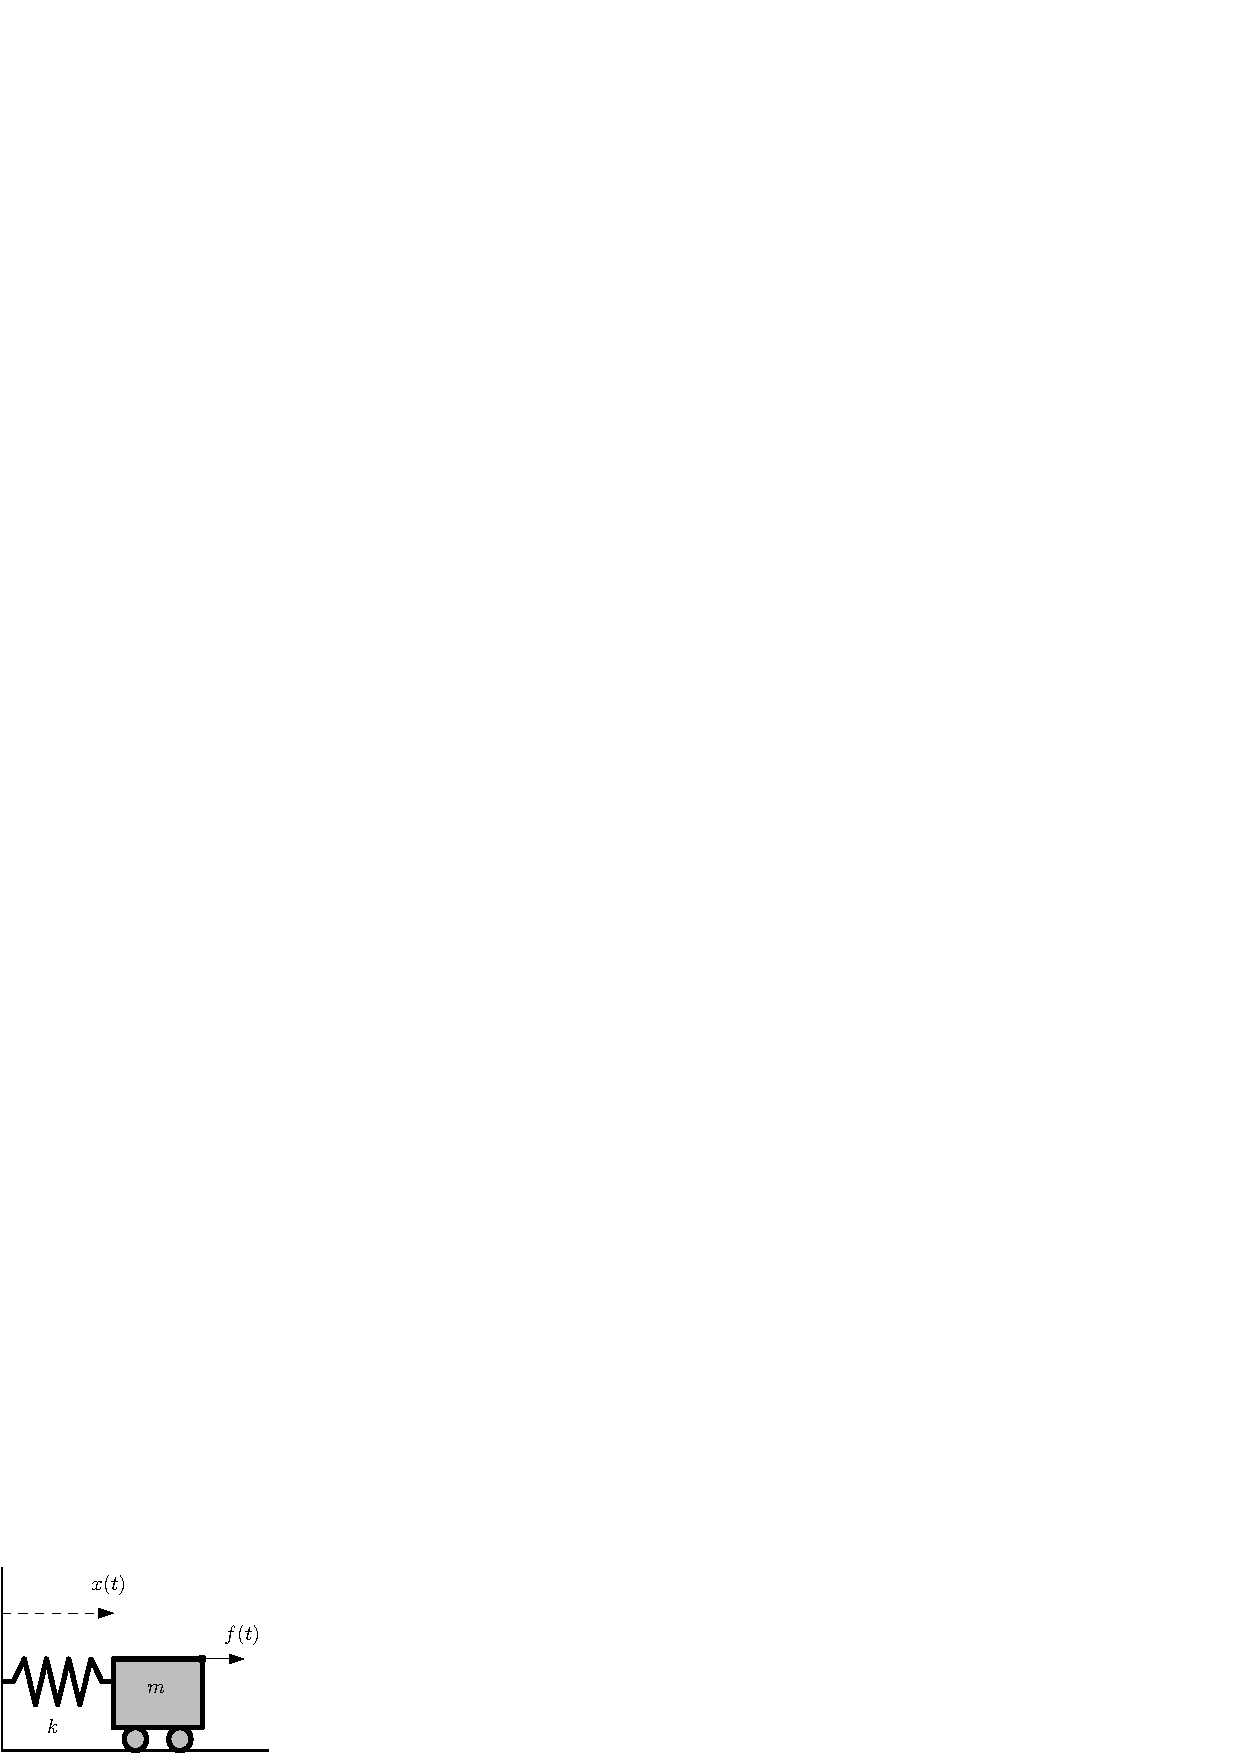
\includegraphics[width=0.75\linewidth]{img/cart.png}
% \end{marginfigure}
% \begin{question}
%   The figure in the margin shows a cart strapped by two elastic springs to walls. Sketch a free-body diagram for the cart and use it to write down the 2nd order \ode{} for position variable \(x\) using Newton's laws of motion. Leave \(f(t)\) as an unknown force function.
%   \solspace{3in}
% \end{question}

% \newpage\begin{sagequestion}
%   The \sage code in the link\footnote{Code for mass-damper-spring oscillator: \\ \url{https://goo.gl/p9EVdC}} computes solutions to the mass-damper-spring\index{mass-damper-spring} mechanical oscillator\index{oscillator} evolving from initial position \(p_{0}\) and initial velocity \(v_{0}\), given by equation:\index{damping}
%   \begin{equation}
%     \label{eq:w5-1}
%     m \ddot x + c \dot x + k x = 0,\quad x(0)=p_{0}, \dot x(0) = v_{0}
%   \end{equation}

%   \begin{enumerate}[(a)]

%   \item Copy the sketch into the graph below. Pay special attention to the
%     points in which either of the functions intersects with the horizontal.

%     \begin{minipage}{0.48\linewidth}
%     \emptygrid{5}{4}
%   \end{minipage}
%     \begin{minipage}{0.48\linewidth}
%   \item What is the position curve doing when the velocity curve intersects the horizontal?
%   \solspace{0.25in}

% \item Are these curves growing, decaying (transient), or neither? Are they oscillating or not?\index{transient}
%   \solspace{0.25in}
% \end{minipage}

% \begin{minipage}{0.48\linewidth}
% \item Slowly increase damping \(c\) by modifying the code until the curves stop oscillating. Try to find the smallest positive \(c\) that stops the oscillations. Then copy the graph into the space on the right and note the value of this \emph{critical damping}\index{damping!critical} \(c\).
% \end{minipage} \begin{minipage}{0.48\linewidth}
% \begin{center}
%     \emptygrid{5}{4}

%     \vspace{1em}
%         Critical \(c = \)
%     \end{center}
%   \end{minipage}
% \end{enumerate}

% \end{sagequestion}

% \begin{question}
%   Verify that \(y(x) = e^{x}\sin(x)\) satisfies \(y''(x) - 2 y'(x) + 2 y(x) = 0\).
% \end{question}
% \solspace{3.5in}

% \begin{question}
% Given a linear \ode{} $y''= y' + 12y$. \index{characteristic equation!real roots}
% \begin{enumerate}[(a)]
% \item Is this equation homogeneous or not? How do you know? \index{homogeneous} \solspace{.25in}
% \item Calculate the general solution of the \ode{}. \solspace{2in}
% \item Calculate $c_1$ and $c_2$ so that $y(0) = 1$, and $y'(\pi) = 0$.\solspace{1.5in}
% \end{enumerate}
% \end{question}

% \begin{question}
%   Compute real and imaginary parts of each of the following expressions\footnote{
%     Product of exponentials:
%     \(e^{a\pm b} = e^{a} e^{\pm b}\)\\
%     Euler's formula: \(e^{\pm i x} = \cos(x) \pm i \sin (x) \)
%     }:
%   \begin{enumerate}[(a)]
%   \item \( \displaystyle (2+i)(3-i)\) \solspace{.5in}
%     \item \( \displaystyle e^{3i}\) \solspace{.5in}
%     \item \( \displaystyle e^{2-i\frac{\pi}{2}}\) \solspace{.5in} \marginnote{A consequence of Euler's formula\index{Euler's formula} is that the \(\cos\) and \(\sin\) functions can be defined using complex exponentials:
%   \begin{align*}
%     \cos(x) &= \frac{1}{2}e^{i x} + \frac{1}{2}e^{-i x} \\
%     \sin(x) &= \frac{1}{2i}e^{i x} - \frac{1}{2i}e^{-i x}
%   \end{align*}
% Compare these formulas with those in the margin of the following page.}

%     \item \( \displaystyle \frac{1}{i}\) \solspace{.5in}
%     \item \( \displaystyle \frac{1}{1-i}\) \solspace{.5in}
%   \end{enumerate}
% \end{question}


% \subsection*{Discussion Problems}

% \begin{question}
%   A particular solution to a second-order \ode{} is given by
%   \[
%     y(x) = 2e^{-3x} + 3 e^{x}
%   \]

%   \begin{enumerate}[(a)]
%   \item Give the initial conditions \(y(0)\) and \(y'(0)\) of the function above.
%   \item Give an example of a \ode{} whose solution is given by the function above.
% \end{enumerate}
% \end{question}

% \begin{question}
%   Calculate general solutions to the following linear \ode{}s, and particular solutions to IVPs where appropriate.
%   \begin{enumerate}[(a)]
%   \item \(\ddot{x} - 2\dot{x} - 3x = 0,\quad x(0) = 0, \dot x(0) = 1\)
%   \item \(\ddot{y} - 5\dot{y} + 6y = 0,\quad y(0) = 1, \dot y(0) = -1\)
%   \item \(y'''(x) - 3y''(x) + 2y'(x) = 0\)
%   \end{enumerate}
% \end{question}

% \begin{question}
%   Compute real and imaginary parts of each of the following numbers:
%   \begin{colenumerate}[3]
%     \item \(-2i(2+3i)\)
%     \item \((1+i)(2+i)\)
%     \item \((2-3i)(2+3i)\)
%     \item \(e^{i \frac{\pi}{4}t}\)
%     \item \(e^{2+i \frac{\pi}{4}}\)
%     \item \(\frac{1}{2+i}  \)
%   \end{colenumerate}
% \end{question}

% \subsection*{Additional practice problems}

% \marginnote{Problems 4.3.38, 41 and 42 are significant. They discuss hyperbolic functions that have definitions similar to \(\cos\) and \(\sin\) in exponential form, except they do not use any complex numbers\index{hyperbolic functions}:
%   \begin{align*}
%     \cosh(x) &= \frac{1}{2}e^{x} + \frac{1}{2}e^{-x} \\
%     \sinh(x) &= \frac{1}{2}e^{i x} - \frac{1}{2}e^{-x}
%   \end{align*}
% Compare these formulas with those in the margin of the previous page and notice that   \begin{align*}
%     \cosh(ix) &= \cos(x) \\
%     i \sinh(ix) &= \sin(x)
%   \end{align*}}

% \begin{colenumerate}
% \item \smallcaps{Zill} \S 4.1.1--4, 29--34
% \item \smallcaps{Zill} \S 4.1.38
% \item \smallcaps{Zill} \S 4.3.1--14, 29--34
% \item \smallcaps{Zill} \S 4.3.41--42
% \end{colenumerate}
% The problems where characteristic equation has complex or repeated roots will be covered on Wed and Fri. You can either wait until we cover these problems in lectures, or read ahead to see what happens in those cases.








% \section{Complex and repeated roots,  Independence of solutions}

% \begin{weekintro}
%   Complex-valued functions\index{complex-valued functions} have real and imaginary parts, just like complex numbers. For functions, real and imaginary parts are functions themselves, that we can sketch. They often have related, but not identical, behaviors. \index{characteristic equation!complex roots}

%   When roots of the characteristic polynomials repeat verbatim, such as in \(M^{2} + 2M + 1 = (M+1)^{2}\), we have to be careful in writing out the solution. These cases require a modification of the solution function in order to obtain the correct general solution.
%   \index{characteristic equation!repeated roots}

% \marginnote{\textbf{Definition} of a concept and \textbf{calculation} are not always equivalent in mathematics. Definition speaks of \emph{meaning}, while calculation tells us \emph{how to compute} something. For example, \emph{definition} of a solution of \(ax^{2} + bx + c = 0\) is ``any number that satisfies the equation'', and the calculation is given by the familiar quadratic formula. For quintic (5th order polynomial), there is no similar formula (calculation) of a solution, just a definition.}  Even though we infer very particular formulas for two functions that solve 2nd order linear \ode{}s, any two functions that are
%   \begin{compactenum}[(i)]
%     \item particular solutions (separately), and
%     \item \textbf{linearly independent} \index{linear independence}
%   \end{compactenum}
%   can be used to form a general solution. What does it mean to be linearly independent? Informally, it means that behavior of one is fundamentally different from the other. A more in-depth definition is in the textbook. To \textbf{check} for linear independence, we use the Wronskian determinant.\index{Wronskian}
% \end{weekintro}

% \subsection*{Homework}


% \begin{question}
%   The complex-valued function\footnote{Notation \(e^{x} = \exp(x)\)}  \(f(t)\) depends on real variable \(t\):
%   \[
% f(t) =    \exp\left[(-1+i2\pi)t\right]
% \]
% \begin{enumerate}[(a)]
% \item Compute the real part of the function \(\Re f(t)\) and the imaginary part \(\Im f(t)\). \solspace{1.5in}
%   \item Sketch the real and imaginary parts for \(0 < t < 3\). Make sure to accurately represent growth/decay of each function, their value at \(t=0\), and points at which the functions intersect with the horizontal axis.

%   \item For what values \(t\) is the function \(f(t)\) purely real (imaginary part is 0) and for what values is it purely imaginary (real part is \(0\))?

%   \vspace{1em}

%   \emptygrid{6}{2} \quad \emptygrid{6}{2}
% \end{enumerate}
% \end{question}

% \begin{question}
%   Compute solutions to the following linear homogeneous \ode{}s. In all cases, use real-valued formulas.
%   \begin{enumerate}[(a)]
%   \item \(y'' + 4y = 0\) \solspace{1in}
%   \item \(y''+2y'+y = 0 \) \solspace{1in}
%   \item \(y''+2y' + 5y = 0\) \solspace{1in}
%   \end{enumerate}
% \end{question}

% \begin{question}
% An unforced response of an oscillator can be modeled using the \ode{} \(m \ddot x(t) + c \dot x(t) + k x(t) = 0\), where \(m\) is the mass, \(c\) is the damping coefficient, and \(k\) the spring stiffness.\index{mass} \index{damping} \index{stiffness}
%   \begin{enumerate}[(i)]
%     \item  For \(m=4\) and \(k = 9\) and undetermined \(c \geq 0\), find the roots of the characteristic equation. \solspace{1in}
%     \item Find the ranges of values of \(c\) such that the general solution is:
%       \begin{inparaenum}[(i)]
%       \item decaying and shows no oscillation,
%       \item decaying and has oscillations.
%       \end{inparaenum} Compare your answer here to the \sage problem in previous week's homework.

%       \solspace{1in}
%     \item Choose one value for each range you determined and write out the formula for the general solution. \solspace{2in}
%     \end{enumerate}
%     \solspace{4in}
% \end{question}

% \subsection*{Discussion Problems}

% \begin{question}
%   Calculate real and imaginary parts of the following functions (\(t\) is always a real number):
%   \begin{colenumerate}[3]
%   \item \((2+i)\cos(t)\)
%   \item \(3i[ \cos(t) - i\sin (t) ]\)
%   \item \(\exp( i2t )\)
%   \item \((2+i)\exp( i2t )\)
%   \item \(\exp(3t-i2t )\)
%   \item \(5e^{(2+i \frac{\pi}{4})t}\)
%   \end{colenumerate}
% \end{question}

% \begin{question}
% Given $y''-2y'+2y = 0$.
% \begin{enumerate}[(a)]
% \item Verify that $y=c_1e^x\cos(x) + c_2 e^x\sin(x)$ is a general solution to the given \ode{}.
% \item Find $c_1$ and $c_2$ so that $y(0) = 1$, and $y'(\pi) = 0$.
% \item Use Wronskian to verify that $e^{x}\cos(x)$ and $e^{x}\sin(x) $ are linearly independent.
% \end{enumerate}
% \end{question}

% \begin{question}
% Find the general (or particular) solution and determine if the solution will exhibit growth or decay.\index{growth} \index{decay}
% \begin{colenumerate}
% \item $y''+8y'+16y = 0$
% \item $y''+2y'+2y = 0$
% \item $y''+2y'-8y = 0$, $y(0) = 7$, $y'(0) = 2$
% \end{colenumerate}
% \end{question}

% \begin{question}
%   For each of the following pairs of numbers:
%   \begin{itemize}
%   \item find quadratic equations with real coefficients that have the following roots,
%   \item describe (oscillating or not, growing/decaying/neither) the shape of solutions of a 2nd order linear \ode{} whose characteristic equation would be given by the quadratic you just found.
%   \end{itemize}
%     \begin{colenumerate}[4]
%     \item \(-2\), \(3\)
%     \item \(0\), \(2\)
%     \item \(2\), \(2\)
%     \item \(\pm i\)
%     \item \(2 \pm i\)
%     \item \(A, B\)
%     \item \(A \pm i B\)
%     \end{colenumerate}
% where \(A, B\) are both real constants.
% \end{question}

% \begin{question}
%   For each of the functions below
%   \begin{compactitem}
%   \item Give the initial conditions \(y(0)\) and \(y'(0)\) of the function above.
%   \item Give an example of a \ode{} whose solution is given by the function above.
%   \end{compactitem}

%   \begin{colenumerate}[2]
%   \item \(y(x) = 2e^{-3x} + 3 e^{x}\)
%   \item \(y(x) = \sin(x) + \cos(x)\)
%   \item \(y(x) = xe^{-2x} -3 e^{-2x}\)
%   \item \(y(x) = e^{-x}\cos(2x)\)
%   \end{colenumerate}
% \end{question}


% \begin{question}
% A mass of  \(4 \si{kg}\) is attached to a spring whose spring constant is 16 \si{kg/s^2}. What is the period of the motion of the mass when it is allowed to bounce freely?
% \end{question}

% \begin{question}
% A mass of \(20 \si{kg}\) is attached to a spring. If the frequency of its free motion is $2/\pi$ cycles/s,
% what is the spring constant $k$? What is the frequency of free motion if the original mass is replaced with an \(80 \si{kg}\) mass?
% \end{question}

% \subsection*{Additional practice problems}

% \begin{compactenum}[(a)]
% \item \smallcaps{Zill} \S 4.1.15--19 (Wronskian, independence of solutions)
% \item \smallcaps{Zill} \S 4.3.1--14, 29--34, 41--42 (homogeneous \ode{}s)
% \item \smallcaps{Zill} \S 5.1.1--12, 17--23 (mass-spring-damper models)
% \end{compactenum}




 






% \section{Undetermined coefficients}

% \begin{weekintro}
%   While characteristic equations are extremely useful for solving homogeneous \ode{}s, they do not help much when solving the inhomogeneous subproblem.\index{inhomogeneous}

%   \emph{Undetermined coefficients}\index{undetermined coefficients} is a technique for making \textbf{educated guesses} about \textbf{candidates} for the inhomogeneous solutions. These candidates have undetermined parameters in them that are computed by plugging the candidate into the DiffEq.

%   \textbf{Rely as little as possible on tables of undetermined coefficients.} Instead focus on three principles:
%   \begin{itemize}
%   \item If the input function is a sum of terms, then we can solve inhomogeneous equations with each of the terms in the sum in isolation, and add their solutions together.
%   \item A good candidate for an inhomogeneous solution is formed by a linear combination of derivatives of the input function.
%   \item If the candidate for inhomogeneous solution matches a component in the \emph{homogeneous} solution, multiply the candidate by the independent variable (repeat if necessary).
%   \end{itemize}

% In a particular case of undamped oscillators, the third principle above corresponds to the \textbf{resonance}: growth of the output despite bounded input.
% \end{weekintro}

% \subsection*{Homework}

% \begin{question}
%   For each of the following, determine the homogeneous solution and the \textbf{form} of a particular non-homogeneous solution:
%   \begin{fullwidth}
%   \begin{colenumerate}[4]
%   \item \(y'' + 4y = x^{2}\)
%   \item \(y'' + 4y = 10 + \sin(x)\)
%   \item \(y'' + 4y = \sin(2 x)\)
%   \item \(y'' + 4y = e^{x}\sin(2 x)\)
% \end{colenumerate}
%   \solspace{1in}
% \end{fullwidth}
% \end{question}

% \begin{question}
% For the differential equation
%   \[
%     y'' + 9y = x + \sin(x)
%   \]
%   \begin{enumerate}[(i)]
%   \item Solve
%     \begin{fullwidth}
%     \begin{colenumerate}[3]
%     \item Homog. Subproblem
%     \item Inhomog. Subproblem 1
%     \item Inhomog. Subproblem 2
%     \end{colenumerate}

%     \solspace{3in}

%     \end{fullwidth}
%     \item General solution using part (i). \solspace{0.5in}
%   \item Particular solution that satisfies \(y(0)=1\), \(y'(0) = 0\). \solspace{2in}
%   \end{enumerate}
% \end{question}

% \begin{question}
% A mass of \(24 \si{kg}\), attached to the end of a spring of unknown coefficient \(k\), stretches it \(4\si{cm}\) under influence of gravity (\(g \approx 10 \si{ms^{-2}}\)) when the mass is not moving.
% \begin{enumerate}[(i)]
%   \item Write the differential equation for the system.
%   \item Compute the equilibrium solution for the equation and determine spring coefficient from it.
%   \item Initially, the mass is released from rest from a point \(3 \si{cm}\) above the equilibrium position. Find the particular solution of the differential equation.
% \item In a second scenario, a periodic force \(\cos(\Omega t)\) is applied to the mass in addition to gravity. What is the value of frequency \(\Omega\) which excites resonance\index{resonance} in the motion of the weight?
% \end{enumerate}
% \end{question}

% \begin{sagequestion}
%   The \sage code in the link is the same as used a couple of weeks ago.\footnote{Code for mass-damper-spring oscillator: \\ \url{https://goo.gl/p9EVdC}} Modify the code so that it corresponds to the differential equation
%   \begin{equation}
%     \label{eq:w7-1}
%     \ddot x + 4 x = \sin( \Omega t ),\quad x(0)=p_{0}, \dot x(0) = v_{0}
%   \end{equation}
%   by changing the line 10 appropriately. \footnote{To represent symbol \(\Omega\) you can add a variable \texttt{Omega} in the same fashion as \texttt{mass}, \texttt{damping}, etc. are defined. Set \(\Omega=1\) initially.}
%   \begin{enumerate}[(a)]

%   \item Copy the sketch for \(\Omega=1\) into the graph below. \footnote{Set \texttt{xmax=20} in lines 22 and 28 and \texttt{ymin=-10} and \texttt{ymax=20} at the end of the code to show you the full extent of solution curves.}

%     \begin{minipage}{0.48\linewidth}
%     \emptygrid{5}{4}
%   \end{minipage}
%     \begin{minipage}{0.48\linewidth}
%   \item Describe how the graphs are different compared to the graphs without \(\sin(\Omega t)\) added (you can look back to Week 5).
%   \solspace{0.25in}

% \item Are these new curves growing, decaying, or neither? Are they oscillating or not?
%   \solspace{0.25in}
% \end{minipage}
% \item Write down the characteristic equation and find its roots. What is the value of the \emph{resonant frequency} of this oscillator?
%   \solspace{.5in}

% \begin{minipage}{0.48\linewidth}
% \item Set \(\Omega\) equal to the \emph{resonant frequency}\index{resonant frequency} of the differential equation. Then copy the graph into the space on the right.

%   Resonant \(\Omega = \)
% \end{minipage} \begin{minipage}{0.48\linewidth}
%   \begin{center}
%     Resonant \(\Omega = \)

%     \emptygrid{5}{4}

%     \vspace{1em}
%         Are the curves growing, decaying, or neither? \index{resonance}
%     \end{center}
%   \end{minipage}
% \end{enumerate}

% \end{sagequestion}


% \subsection*{Discussion and Practice Problems}

% \begin{question}
%   In each of the following equations, undetermined coefficient candidate for the inhomogeneous solution is incorrectly proposed.
%   \begin{compactitem}
%   \item Proceed with the incorrect candidate and \textbf{show how the solution process fails}.
%   \item \textbf{Propose the correct undetermined coefficients candidate}.
%   \item \textbf{Find the coefficients} of the inhomogeneous solution.
%   \end{compactitem}
%  \begin{enumerate}[(a)]
%   \item \(y'' + 2y' + 5y = x^{2}\), incorrect candidate: \(y_{p}(x) = A x^{2} + B\)
%   \item \(y'' + 9 y = \sin(x)\), incorrect candidate: \(y_{p}(x) = A \sin(x)\)
%   \item \(y'' + 9 y = \sin(3x)\), incorrect candidate: \(y_{p}(x) = A \cos(3x) + B\sin(3x)\)
% \end{enumerate}
% \end{question}

% \begin{question}
% For each of the following, determine the homogeneous solution and the \textbf{form} of a particular non-homogeneous solution:
%   \begin{colenumerate}
%   \item $y''+3y'+2y = -10x^2$
%   \item $y''+3y'+2y =e^{4x}$
%   \item $y''+2y'=x^2+5x$
%   \item $y''+4y'+13y = 2xe^{-2x}\sin(3x)$
%   \item $y''+2y'+2y=5e^{-x}\cos(x)$
%   \item $y''+6y'+9y = x^3e^{-3x}$
%   \end{colenumerate}
% \end{question}

% \begin{question}
% Using the method of undetermined coefficients to find the general solution:
%   \begin{enumerate}[(i)]
%   \item $y''+3y'+2y=-10x^2$
%   \item $y''+3y'+2y =e^{4x}$
%   \item $y''+y'-2y = 20\sin(2x)$
%   \item $y'''-2y''+y' = 2-24 e^x +40 e^{5x}$, $y(0) = 1/2, y'(0)=5/2, y''(0) = -9/2$.
%   \end{enumerate}
% \end{question}

% \begin{question}
% A weight of \(8 \si{kg}\) hung from a spring stretches the spring \(3\si{cm}\). The mass-spring system is additionally encumbered by air resistance, which is proportional to velocity with coefficient \(1 \si{kg/s}\). The mass moves under the influence of gravity (\(g \approx 10 ms^{-2}\)) and an external force of $10\cos(4t) \si{kgms^{-2}}$ (t is seconds
% after the release). If the weight is pulled down \(1 \si{m}\) from its equilibrium position
% and given an initial upward velocity of \(2 \si{m/s}\), write an initial value problem for the position of
% the object at time t seconds and solve.
% \end{question}

% \subsection*{Additional practice problems}


% \begin{colenumerate}
%   \item \smallcaps{Zill} \S 4.4.1--15, 27--32 (undet. coeff)
%   \item \smallcaps{Zill} \S 5.1.29--34 (forced oscillator)
%   \item \smallcaps{Zill} \S 5.1.37--38 (resonance)
% \end{colenumerate}












% \section{Practice for test --- Higher order linear ODEs}

% There is no homework due in this discussion. Instead, study from the previous weeks and additionally work through problems below \textbf{before} you come to the discussion. The TA will cover the questions you struggle with.

% You can use the following step-by-step calculator to help you study: \url{https://goo.gl/sZEyvL}. Do not rely on it too much, though, as you will not have such help in an exam.

% \begin{question}
%   Find the general solution of the following \ode{} by completing each of the subparts.
%   \[
%     \frac{1}{5}y''(x) + \frac{4}{5} y'(x) + 4 y(x) =  4x^{2}.
%   \]

%   \begin{enumerate}[(a)]
%   \item Put the equation into the standard form and circle the input function \(f(x)\).
%   \item Find the solution to the homogeneous subproblem.
%   \item According to undetermined coefficients prescription, formulate the \textbf{candidate forced (inhomogeneous) solution} for the inhomogeneous subproblem. \textbf{Explain why you chose that form.}
%   \item Use the solution candidate to find a forced (inhomogeneous) solution.
%   \item Use the forced solution and the homogeneous solution to formulate the general solution.
%     \item Give an example of an input function \(f(x)\) that would result in \emph{resonance} occuring. What would the candidate forced solution look like in that case?
%   \end{enumerate}
% \end{question}


% \begin{question}
%   Verify that the functions \(\cos(\ln(x))\), \(\sin(\ln(x))\) are a fundamental solution set for \( x^{2} y'' + xy' + y = 0, \quad x > 0,\)
%   and form the general solution for the \ode{}.
% \end{question}

% \begin{question}
% For each of the following \ode{}s, use any technique appropriate  to find the \textbf{general solution}. Then  use the initial condition to find the \textbf{particular solution}. Avoid using imaginary numbers in your solution (that is, use \(\cos\) and \(\sin\) functions when appropriate).
%     \begin{enumerate}[(a)]
% \item \( 3y'' - 21y' + 30y = 2 + t^{2} + t\), \(y(0) = 1, y'(0) = 1 \)
% \item \( 3y'' - 30y' + 75y = 6 x \sin(x)\), \(y(0) = 0, y'(0) = 1 \)
% \item \( y'' - 4 y = x^{-1}e^{2x} \), \(y(1) = 1, y'(1) = 1 \)
% \item \( 3y'' - 30y' + 87 = 3 + 6\cos(3x)\), \(y(0) = -1, y'(0) = 0 \)
% \end{enumerate}

% \end{question}

% \begin{question}
% Which of the following three \ode{}s models resonance?  Find forced (inhomogeneous) solution of each of the three equations and sketch them.
%   \begin{enumerate}[(a)]
%   \item \(y'' + 4y = \sin(x)\)
%   \item \(y'' + 4y = e^{x}\sin(2x)\)
%   \item \(y'' + 4y = \sin(2x)\)
%   \end{enumerate}

% \end{question}

% \subsection{Additional practice problems}
